\section{Galilean transformation}
	Suppose an event occurs at some point in space, and it is being observed from two different frames of reference. The we would have two different sets of coordinates which correspond to the same event, as observed from both frames of reference. The set of equations that relate these two sets of coordinates are known as \emph{transformation equations}, because they enable us to \emph{transform} a set of coordinates in one system to another set of coordinates in a different system.
	
	The set of equations used to convert the space and time coordinates of a particle from one inertial frame of reference to another moving at a constant relative velocity is known as a \emph{Galilean transformation}.
	
	\begin{figure}[h!]
		\centering
		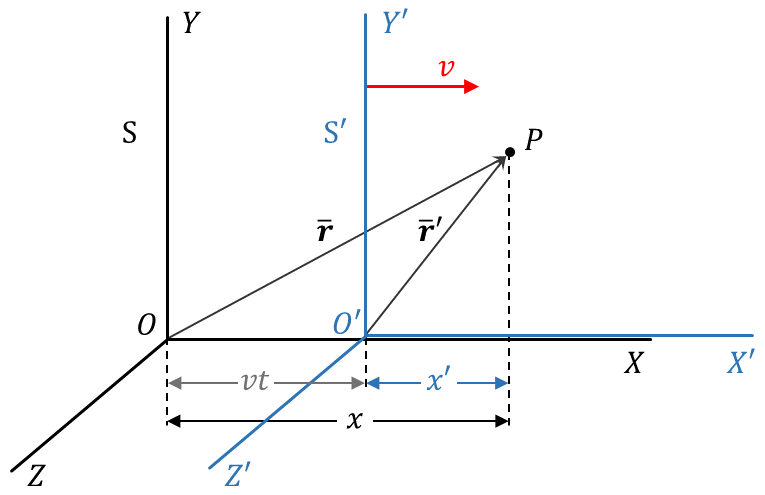
\includegraphics[width=0.6\textwidth]{figures/fig_galilean-transformation-01.png}
	\end{figure}
	
	Let $S$ and $S'$ be two inertial frames of reference whose axes and origins coincide and clocks are synchronized at $t=0$. Suppose the frame $S'$ is moving along the positive $X$ direction with a constant relative speed $v$ with respect to the frame $S$. Then, at some arbitrary time $t$, the separation between the frames is $vt$.
	
	Now, suppose some event occurs at the position $P$ at time $t$. Then $\vb{r}$ and $\vb{r}'$ are the position vectors of the same event with respect to the frames $S$ and $S'$ respectively. If $x$ and $x'$ are the $X$-coordinates of $P$ with respect to $S$ and $S'$ respectively, then they are related as
	\begin{align*}
		x&=x'+vt
	\end{align*}
	Also, because there is no relative motion between the frames along the $Y$ and $Z$ directions, these coordinates with respect to the two frames would be
	\begin{align*}
		y=y'\qq{and}z=z'
	\end{align*}
	Finally, because the clocks of both frames are synchronized, they measure identical times, and so we would have
	\begin{align*}
		t=t'
	\end{align*}
	
	Therefore, the four \emph{Galilean transformation equations} to transform from frame $S$ to frame $S'$ are
	\begin{empheq}[box=\fbox]{align*}
		x'&=x-vt \\
		y'&=y \\
		z'&=z \\
		t'&=t
	\end{empheq}
	In vector form, the above transformation equations may be combined as
	\begin{align*}
		\Aboxed{\vb{r}'&=\vb{r}-\vb{v}t}
	\end{align*}
	
	The four \emph{inverse Galilean transformation equations} to transform from frame $S'$ to frame $S$ are
	\begin{empheq}[box=\fbox]{align*}
		x&=x'+vt' \\
		y&=y' \\
		z&=z' \\
		t&=t'
	\end{empheq}
	In vector form, the above inverse transformation equations may be combined as
	\begin{align*}
		\Aboxed{\vb{r}&=\vb{r}'+\vb{v}t'}
	\end{align*}
	
	\subsection{Galilean invariance}
		When a physical quantity has the same value in two frames of reference, we say that the quantity is \emph{invariant} to a transformation between the frames.
		
		\setcounter{equation}{0}
		\subsubsection{Transformation of length}
			Consider a rod with ends $A$ and $B$, which is being observed with respect to two inertial frames $S$ and $S'$. The frame $S'$ is moving with a constant speed $v$ relative to the frame $S$ along the positive $X$ direction.
			\begin{figure}[h!]
				\centering
				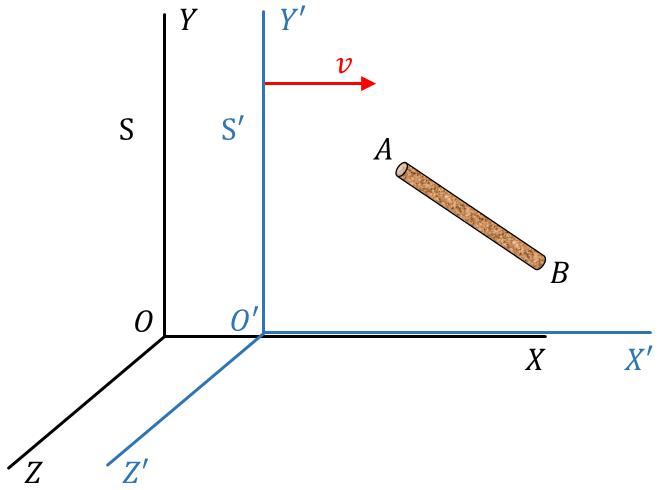
\includegraphics[width=0.5\textwidth]{figures/fig_gal-inv_length.png}
			\end{figure}
			
			In the frame $S$, the coordinates of the ends of the rod are:
			\begin{align*}
				A&:\;(x_A, y_A, z_A) \\
				B&:\;(x_B, y_B, z_B)
			\end{align*}
			
			Likewise, in the frame $S'$, the coordinates of the ends of the rod are:
			\begin{align*}
				A&:\;(x_A', y_A', z_A') \\
				B&:\;(x_B', y_B', z_B')
			\end{align*}
			
			The length of the rod is the distance between $A$ and $B$. Hence in the frame $S$, we have
			\begin{align}
				L&=\sqrt{(x_A-x_B)^2+(y_A-y_B)^2+(z_A-z_B)^2} \label{eqn:gal-inv:L}
			\end{align}
			
			Similarly, in the frame $S'$, we have
			\begin{align}
				L'&=\sqrt{(x'_A-x'_B)^2+(y'_A-y'_B)^2+(z'_A-z'_B)^2} \label{eqn:gal-inv:L-p}
			\end{align}
			
			Now, from the Galilean transformation of the coordinates of $A$ and $B$, we have
			\begin{align*}
				x'_A&=x_A-vt,\;y'_A=y_A,\;z'_A=z_A \\
				x'_B&=x_B-vt,\;y'_B=y_B,\;z'_B=z_B
			\end{align*}
			
			Using the above in equation (\ref{eqn:gal-inv:L-p}), we get
			\begin{align*}
				L'&=\sqrt{[(x_A-vt)-(x_B-vt)]^2+(y_A-y_B)^2+(z_A-z_B)^2} \\
					&=\sqrt{[x_A-\cancel{vt}-x_B-\cancel{vt}]^2+(y_A-y_B)^2+(z_A-z_B)^2} \\
					&=\sqrt{(x_A-x_B)^2+(y_A-y_B)^2+(z_A-z_B)^2} \\
				\implies\Aboxed{L'&=L}\qq{[using eqn. (\ref{eqn:gal-inv:L})]}
			\end{align*}
			
			The above equation shows us that \emph{length or distance between two points remains invariant to a Galilean transformation}.
		
		\subsubsection{Transformation of velocity}
		
		\subsubsection{Transformation of acceleration}